\begin{figure}[htbp]
\centering
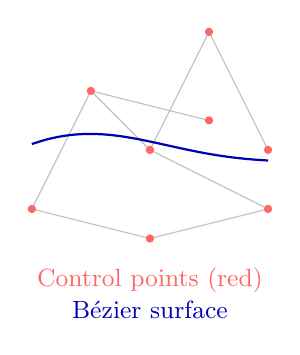
\begin{tikzpicture}[scale=0.75]
  \draw[gray!50,thin] (0,0)--(1,2)--(2,1)--(3,3)--(4,1);
  \draw[gray!50,thin] (0,0)--(2,-0.5)--(4,0);
  \draw[gray!50,thin] (1,2)--(3,1.5);
  \draw[gray!50,thin] (2,1)--(4,0);
  \foreach \x/\y in {0/0, 1/2, 2/1, 3/3, 4/1, 2/-0.5, 4/0, 3/1.5} {
    \fill[red!60] (\x,\y) circle (2pt);
  }
  \draw[blue!70!black,thick] plot[smooth,domain=0:4,samples=20] (\x,{0.8+0.5*sin(\x*40)+0.3*cos(\x*60)});
  \node[font=\small,red!60] at (2,-1.2) {Control points (red)};
  \node[font=\small,blue!70!black] at (2,-1.7) {B\'ezier surface};
\end{tikzpicture}
\caption{B\'ezier surface: a tensor-product surface defined by a control net of points.}
\label{fig:bezier_surface}
\end{figure}
